\begin{figure}[t]
\centering
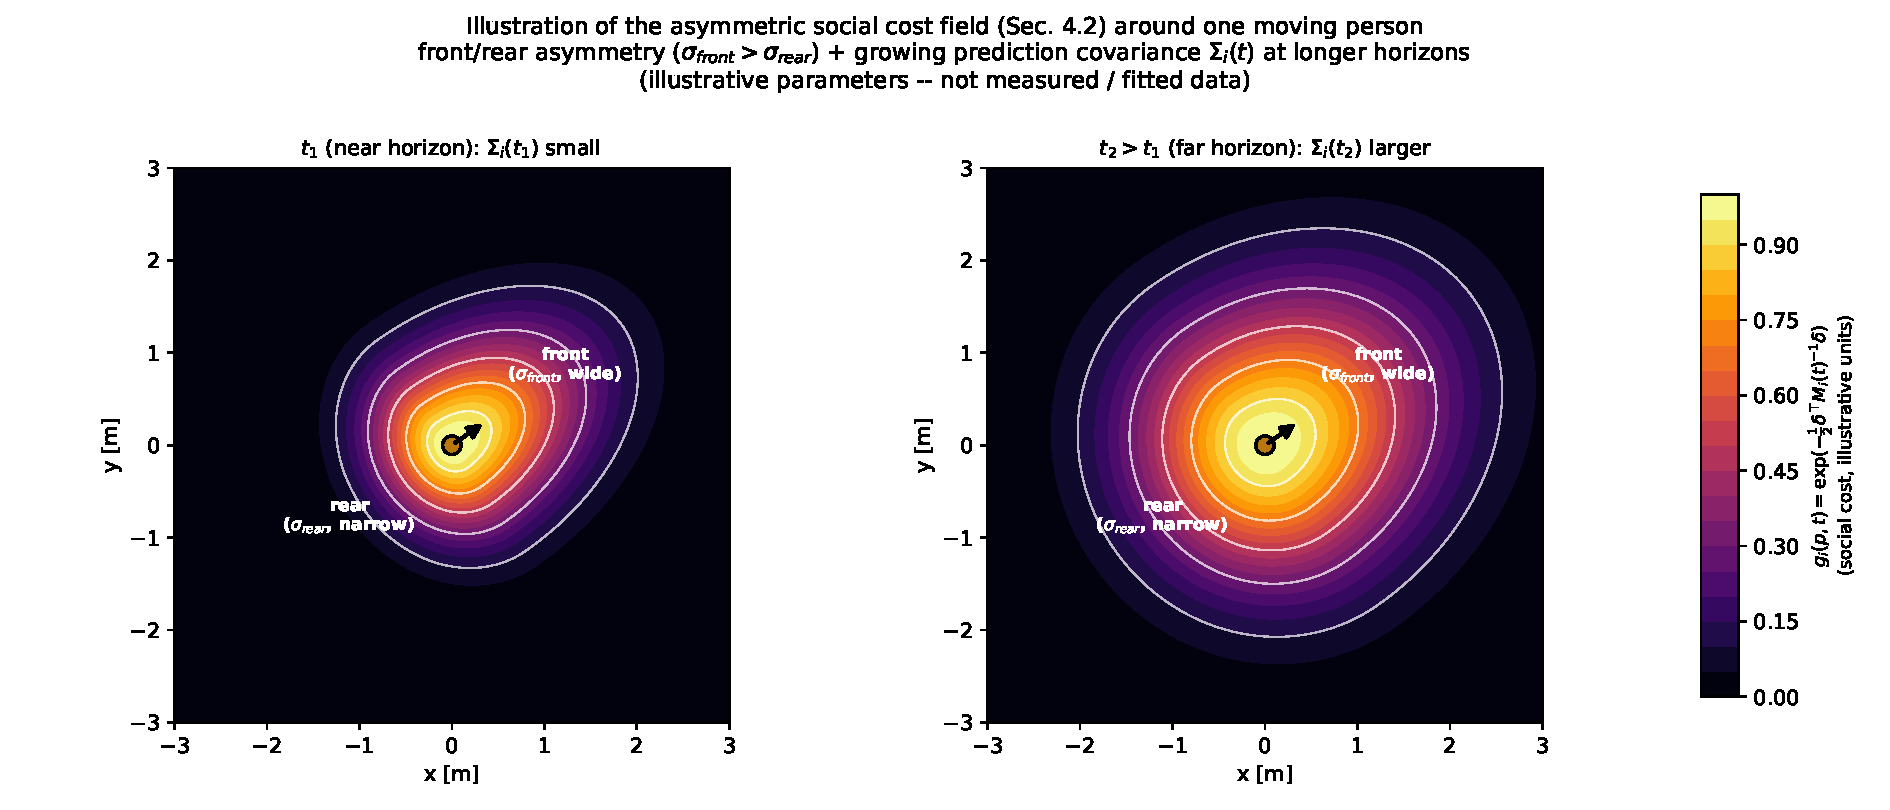
\includegraphics[width=0.85\linewidth]{figures/fig_social_cost_field.pdf}
\caption{\textbf{Asymmetric social cost field} of \cref{subsec:cost}, $g_i(p,t) = \exp(-\tfrac12 \delta^\top M_i(t)^{-1}\delta)$ (a schematic based on the formula, not measured data). Left: near horizon $t_1$ (small predictive covariance $\Sigma_i(t_1)$); right: far horizon $t_2 > t_1$ ($\Sigma_i(t_2)$ grows, expanding the personal-space ellipse). Both panels show the front/rear asymmetry $\sigma_{\text{front}} > \sigma_{\text{rear}}$ (front personal space wider than rear), with half-plane assignment determined by projecting $\delta$ into local coordinates referenced to the person's heading.}
\label{fig:socialcost}
\end{figure}
